\section{Tasks \#1. Freelook and spectral files.}

\subsection{Colorchecker 121 ms}

\subsubsection{Gray scale preview}
Wavelength 429 nm was selected for the gray scale preview. The
preview of the colorchecker and the spectra are shown in Figure
\ref{fig:cc-gray}.

\begin{figure}[H] %
  \centering
  \subfloat[On blue colored area]{%
    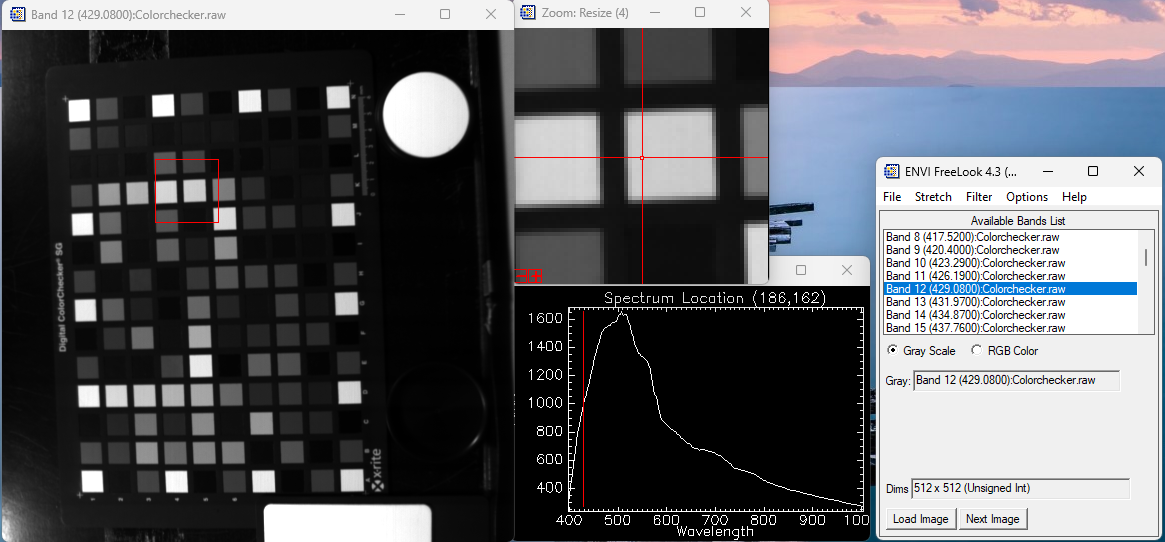
\includegraphics[width=0.45\textwidth]{
      figs/colorchecker_freelook_gray_blue.png
    }
  }
  \hspace{0.1cm}
  \subfloat[On pink colored area]{%
    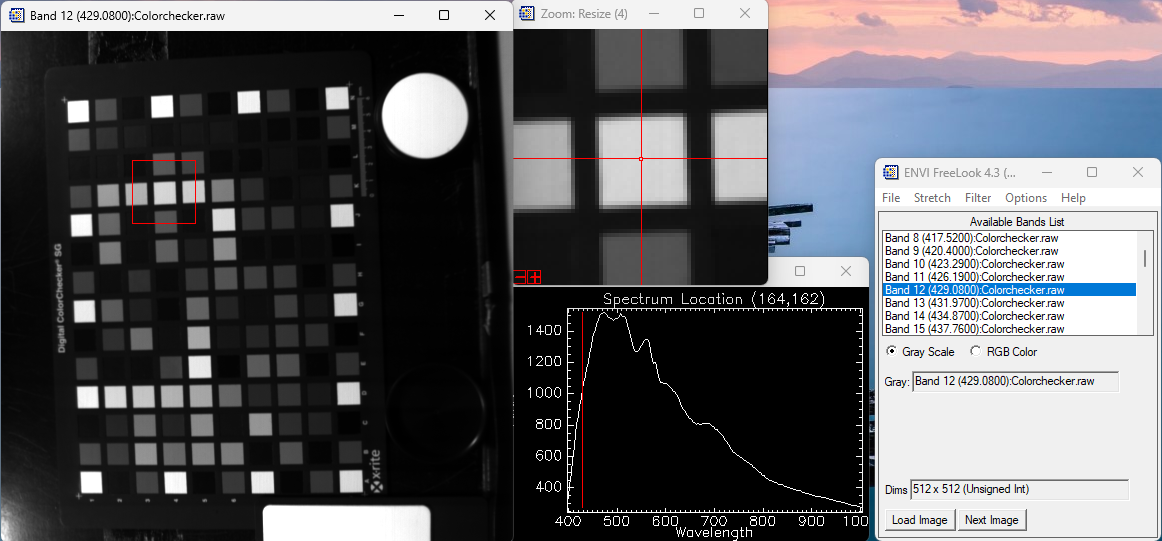
\includegraphics[width=0.45\textwidth]{
      figs/colorchecker_freelook_gray_pink.png
    }
  }
  \caption[]{Gray preview of colorchecker and spectra }
  \label{fig:cc-gray}
\end{figure}

\subsubsection{RGB preview}
Wavelengths 429 nm, 533 nm, and 631 nm were selected for the RGB
preview. The preview of the colorchecker and the spectra are shown in
Figure \ref{fig:cc-rgb}. White correction was not applied to the
spectra. Thus, the color of these images is "natural".

\begin{figure}[H] %
  \centering
  \subfloat[On blue colored area]{%
    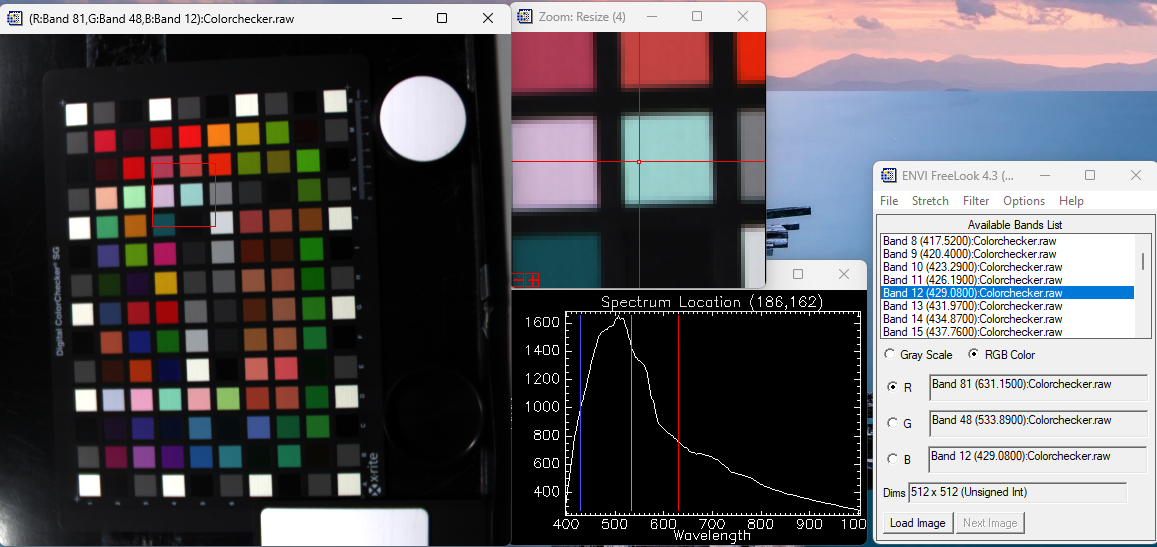
\includegraphics[width=0.45\textwidth]{
      figs/colorchecker_freelook_rgb_blue.png
    }
  }
  \hspace{0.1cm}
  \subfloat[On pink colored area]{%
    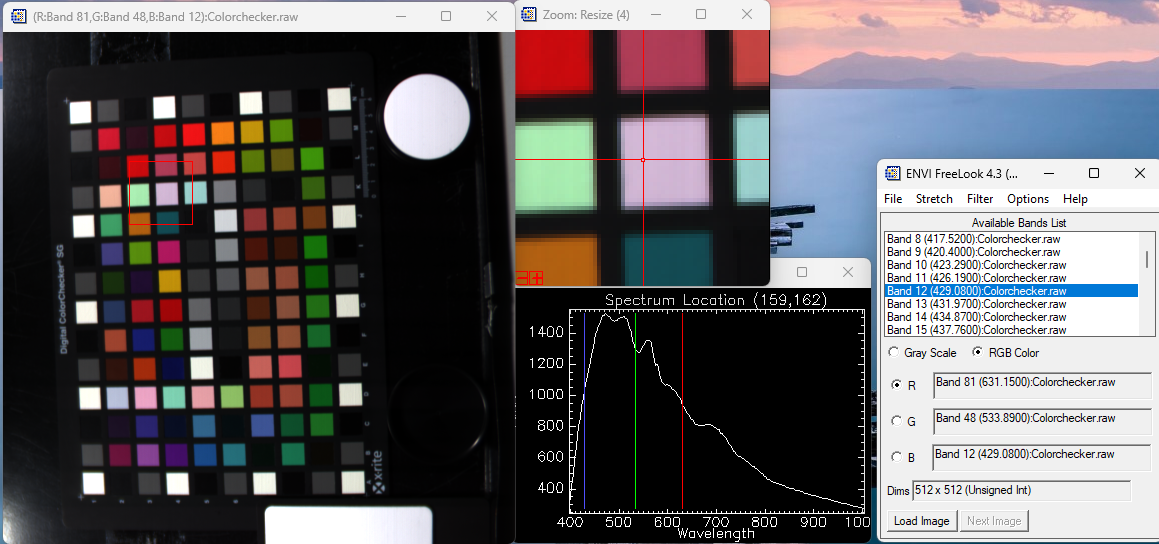
\includegraphics[width=0.45\textwidth]{
      figs/colorchecker_freelook_rgb_pink.png
    }
  }
  \caption[]{RGB preview of colorchecker and spectra }
  \label{fig:cc-rgb}
\end{figure}

\subsection{Leaves (Specim IQ)}

The spectral images of live and plastic leaves are shown in Figure
\ref{fig:leaves}.

Wavelength 750 nm was selected for the gray scale preview.
Wavelengths 429 nm, 533 nm, and 750 nm were selected for the RGB preview.

At 750 nm, plastic leaves and live leaves have different reflectance.
The plastic leaves have higher reflectance than the live leaves. This
is because the plastic leaves are more reflective in the near-infrared region.

\begin{figure}[H] %
  \centering
  \subfloat[Gray scale preview]{%
    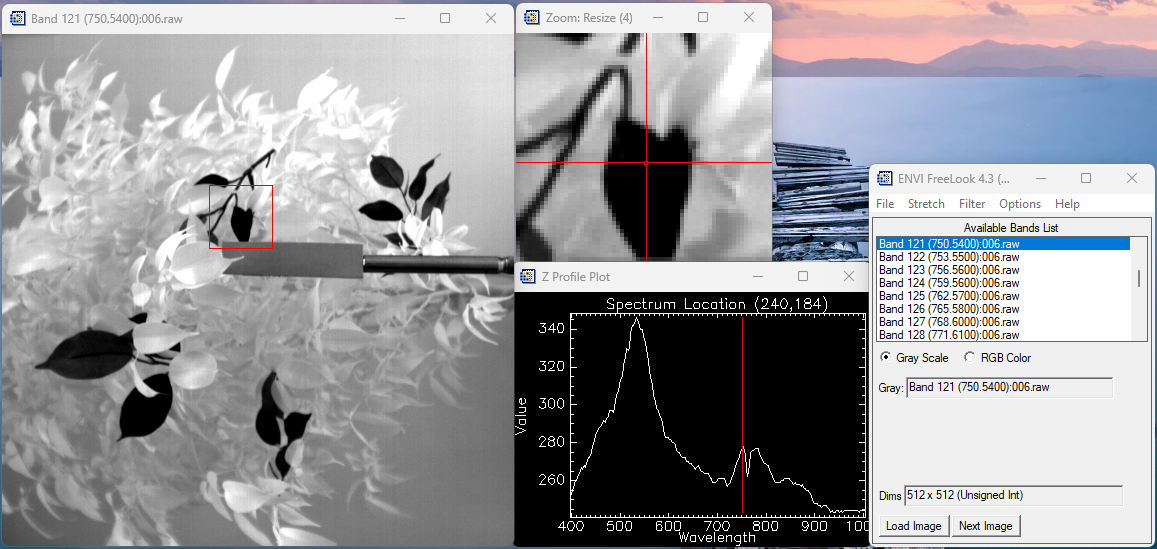
\includegraphics[width=0.45\textwidth]{
      figs/leaves_gray.png
    }
  }
  \hspace{0.1cm}
  \subfloat[RGB scale preview]{%
  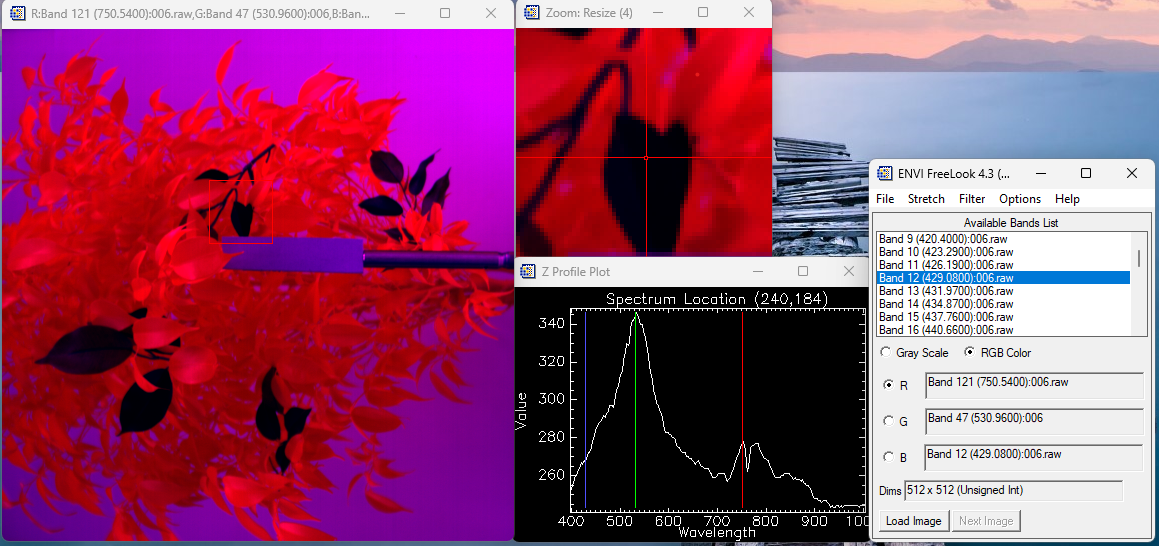
\includegraphics[width=0.45\textwidth]{figs/leaves_rgb.png}}
  \caption[]{Spectral image of live and plastic leaves }
  \label{fig:leaves}
\end{figure}

\subsection{Infrared (by sarita.keski-saari@uef.fi)}

The figure \ref{fig:painting} shows an RGB preview of a painting.
This image was captured with infrared wavelength range. Three
wavelength, 2399 nm, 1496 nm, and 1275 nm were selected to construct
the RGB preview. This is why the preview does not look "natural".

The original RGB picuture of this painting is shown in Figure
\ref{fig:painting-org}.
In Figure \ref{fig:painting}, some obstacles like stamp of coffee cup
are visible. Using infrared spectral image, we can observe hidden
features, not only paintings in visible range.

\begin{figure}[H]
  \centering
  \caption{Infrared spectral image of a painting}
  \label{fig:painting}
  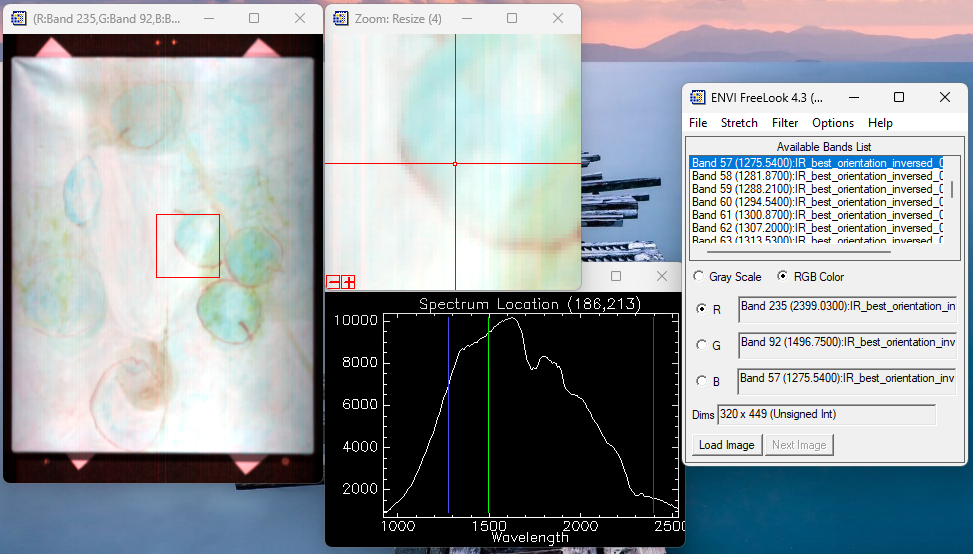
\includegraphics[width=0.5\textwidth]{./figs/painting.png}
\end{figure}

\begin{figure}[H]
  \centering
  \caption{Original RGB view of the paingin}
  \label{fig:painting-org}
  \includegraphics[width=0.5\textwidth]{./figs/painting_visible.png }
\end{figure}

\subsection{124 (rock painting)}

The rock painting has inked areas and other areas. The spectra of
inked areas and other areas are shown in Figure \ref{fig:rock-painting}.

Right-side of Figure \ref{fig:rock-painting-ink1} and Figure
\ref{fig:rock-painting-ink2} shows the spectra of inked areas. These
two spectras have similar distribution compared to the spectra of
rock surface shown in Figure \ref{fig:rock-painting-other}. Thus, we
can say that painted areas have same ink.

\begin{figure}[H]
  \centering
  \subfloat[Spectra of inked area]{
    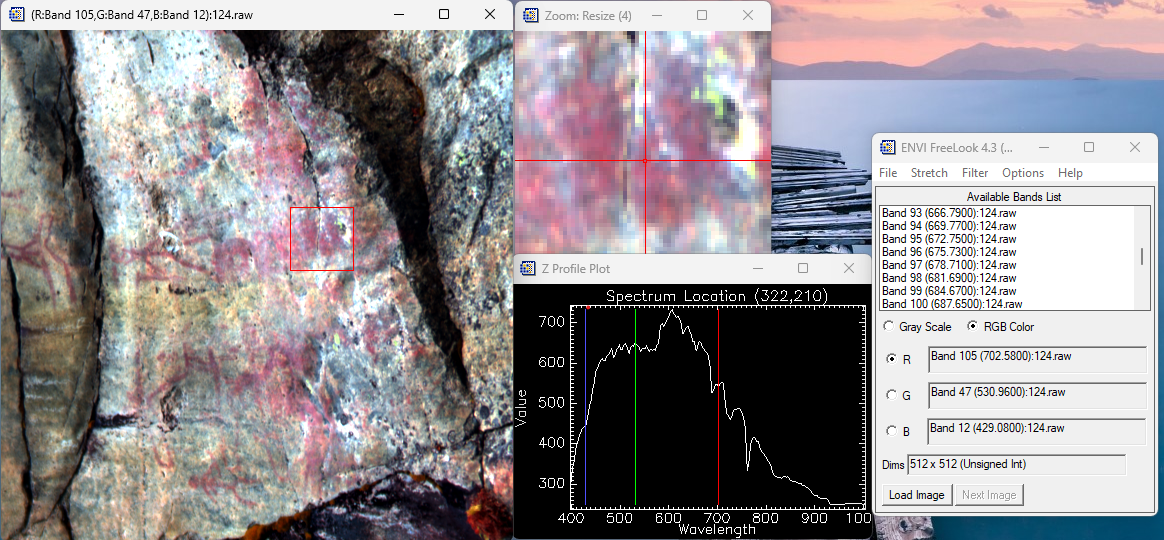
\includegraphics[width=0.45\textwidth]{figs/rock_painting_ink1.png}
    \label{fig:rock-painting-ink1}
  }
  \hspace{0.1cm}
  \subfloat[Another inked area]{
    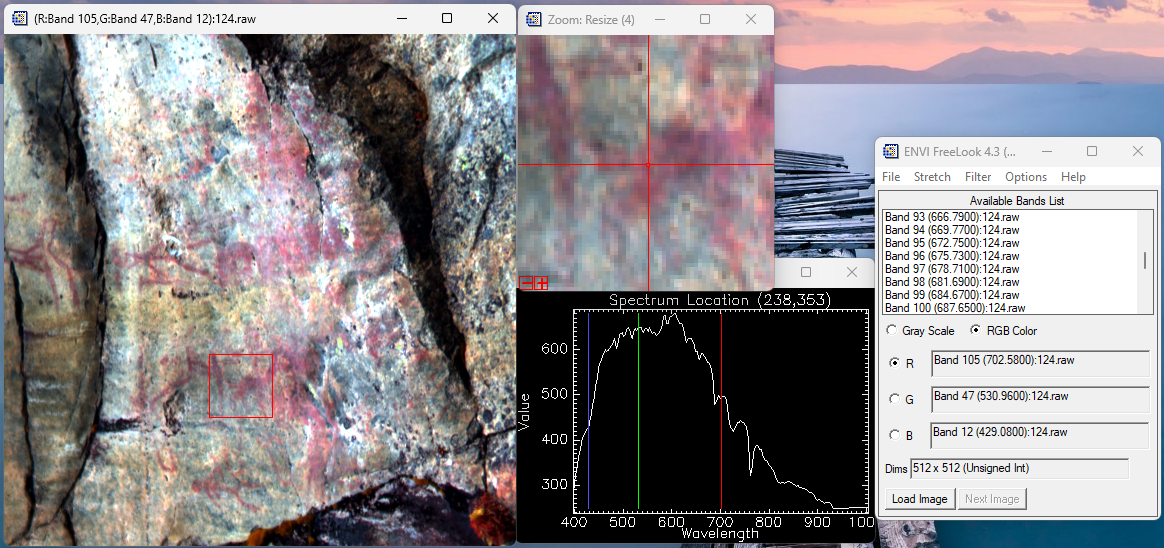
\includegraphics[width=0.45\textwidth]{figs/rock_painting_ink2.png}
    \label{fig:rock-painting-ink2}
  }
  \vspace{0.1cm}
  \subfloat[Spectra of rock surface]{
    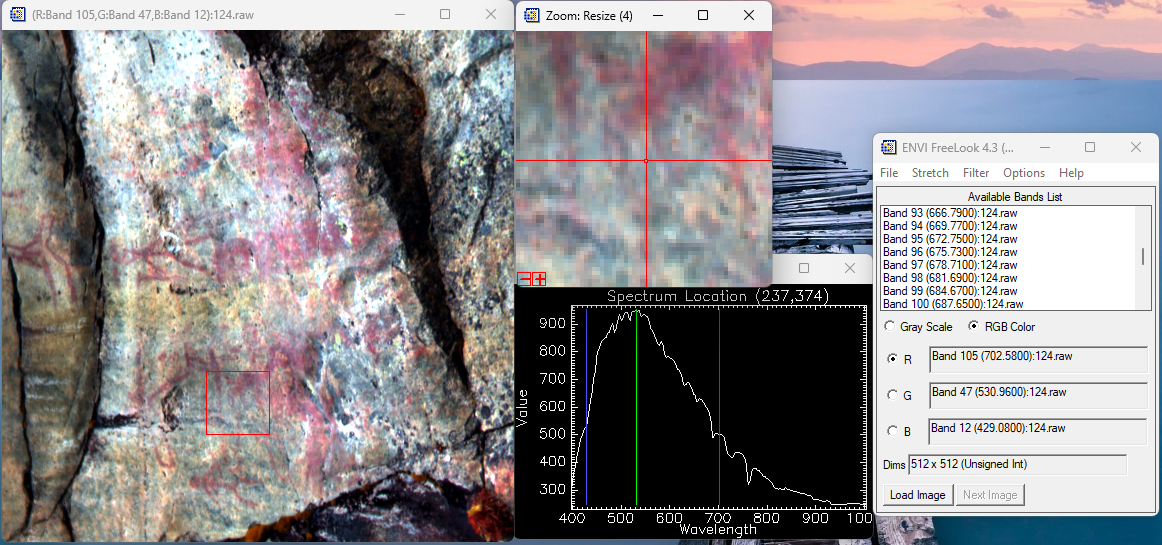
\includegraphics[width=0.45\textwidth]{figs/rock_painting_other.png}
    \label{fig:rock-painting-other}
  }
  \caption[]{RGB preview of rock paintings and spectra }
  \label{fig:rock-painting}
\end{figure}

\section{Tasks \#2. Study csv spectra of different materials}

\subsection{Comparison of two materials}

In Figure \ref{fig:2mat}, the spectras of two materials are compared.
The first comparison is between green paper and yellow paper (Figure
\ref{fig:g-vs-y}). The second comparison is between thin green paper
and green paper (Figure \ref{fig:g-vs-tg}). The green paper has
higher reflectance than the yellow paper in infrared range and has a
peak around 500 nm. The thin green paper has lower reflectance than
the green paper. The thin green paper has a similar reflectance
distribution to the green paper, but the reflectance is lower.

These figures are generated by the code shown in Code \ref{code:comparison}.

\begin{figure}[H] %
  \centering
  \subfloat[Green paper vs yellow paper]{%
    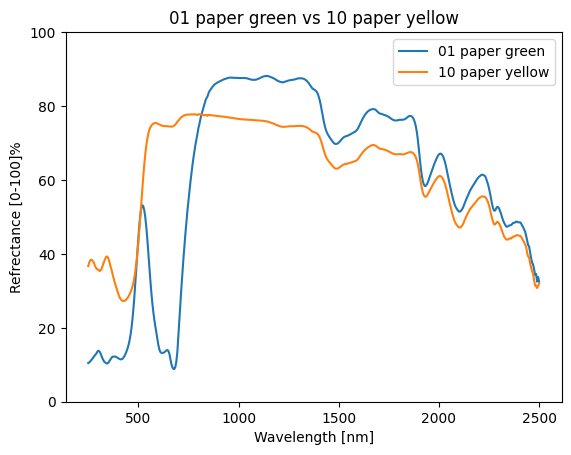
\includegraphics[width=0.45\textwidth]{./figs-task2/2spec-1.png}
    \label{fig:g-vs-y}
  }
  \vspace{0.1cm}
  \subfloat[Thin green paper vs green paper]{%
    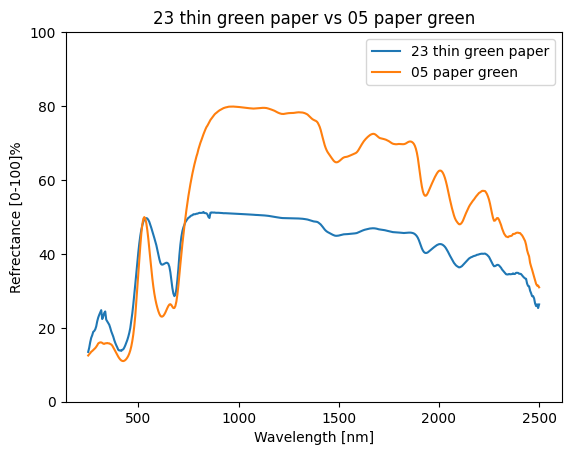
\includegraphics[width=0.45\textwidth]{./figs-task2/2spec-2.png}
    \label{fig:g-vs-tg}
  }
  \caption[]{Comparisons of two materials}
  \label{fig:2mat}
\end{figure}

\subsection{Diffrence of spectra of two materials}
Figure \ref{fig:diff2mat} shows the difference of two materials. This
plot was created by the code shown in Code
\ref{code:compare-materials}. The difference between a green plastic
spoon and a green paper is shown in the figure. The green plastic
spoon has higher reflectance than the green paper in the visible
range. The green paper has higher reflectance than the green plastic
spoon in the infrared range.

\begin{figure}[H]
  \centering
  \caption{Diffrence of two materials}
  \label{fig:diff2mat}
  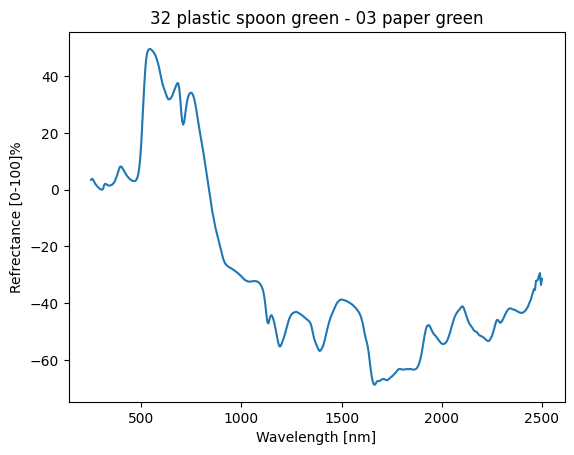
\includegraphics[width=0.5\textwidth]{./figs-task2/2spec-diff.png}
\end{figure}

\subsection{Clustering of all materials by Ward's method}
Figure \ref{fig:clustering} shows the clustering of all materials by
Ward's method. The clustering was done in the visible and infrared
wavelength range. The clustering was done by the code shown in Code
\ref{code:cluster-materials}.

In visible range, green paper and green plastic spoon are clustered
together. In infrared range, green paper and green plastic spoon are
not in the same cluster. This is because the green paper and green
plastic spoon have different reflectance in the infrared range as
shown in Figure \ref{fig:diff2mat}.

\begin{figure}[H] %
  \centering

  \subfloat[Infrared range]{%
    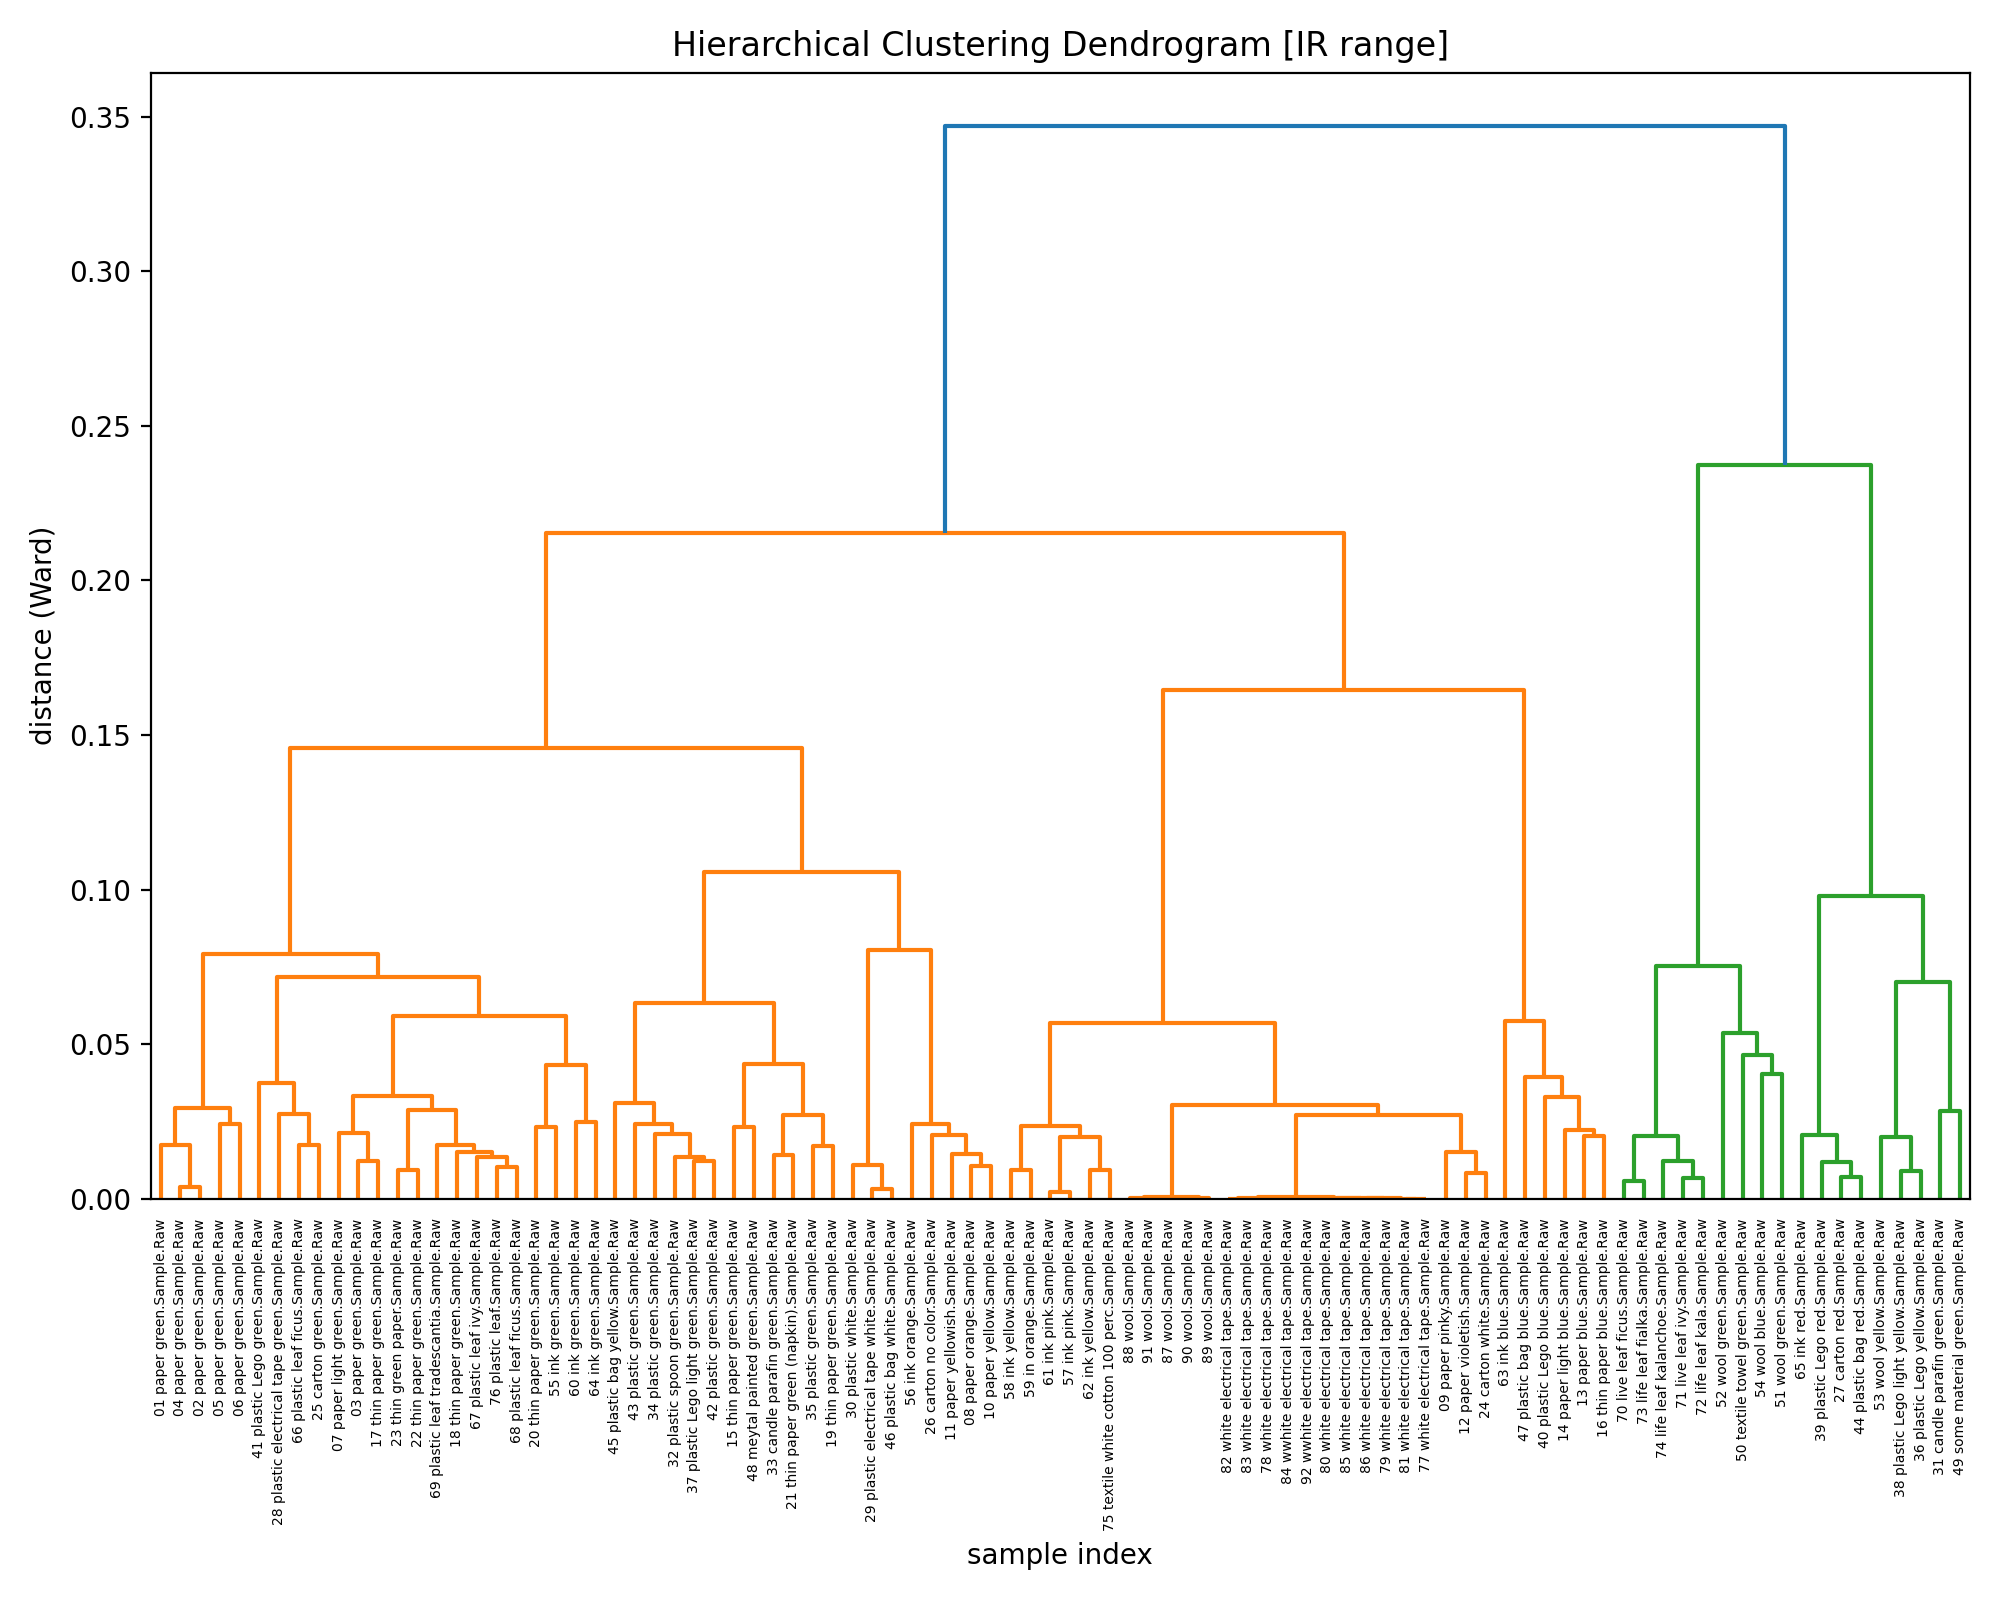
\includegraphics[width=0.65\textwidth]{figs-task2/cluster-ir.png}
  }

  \hspace{0.1cm}

  \subfloat[Visible range]{%
    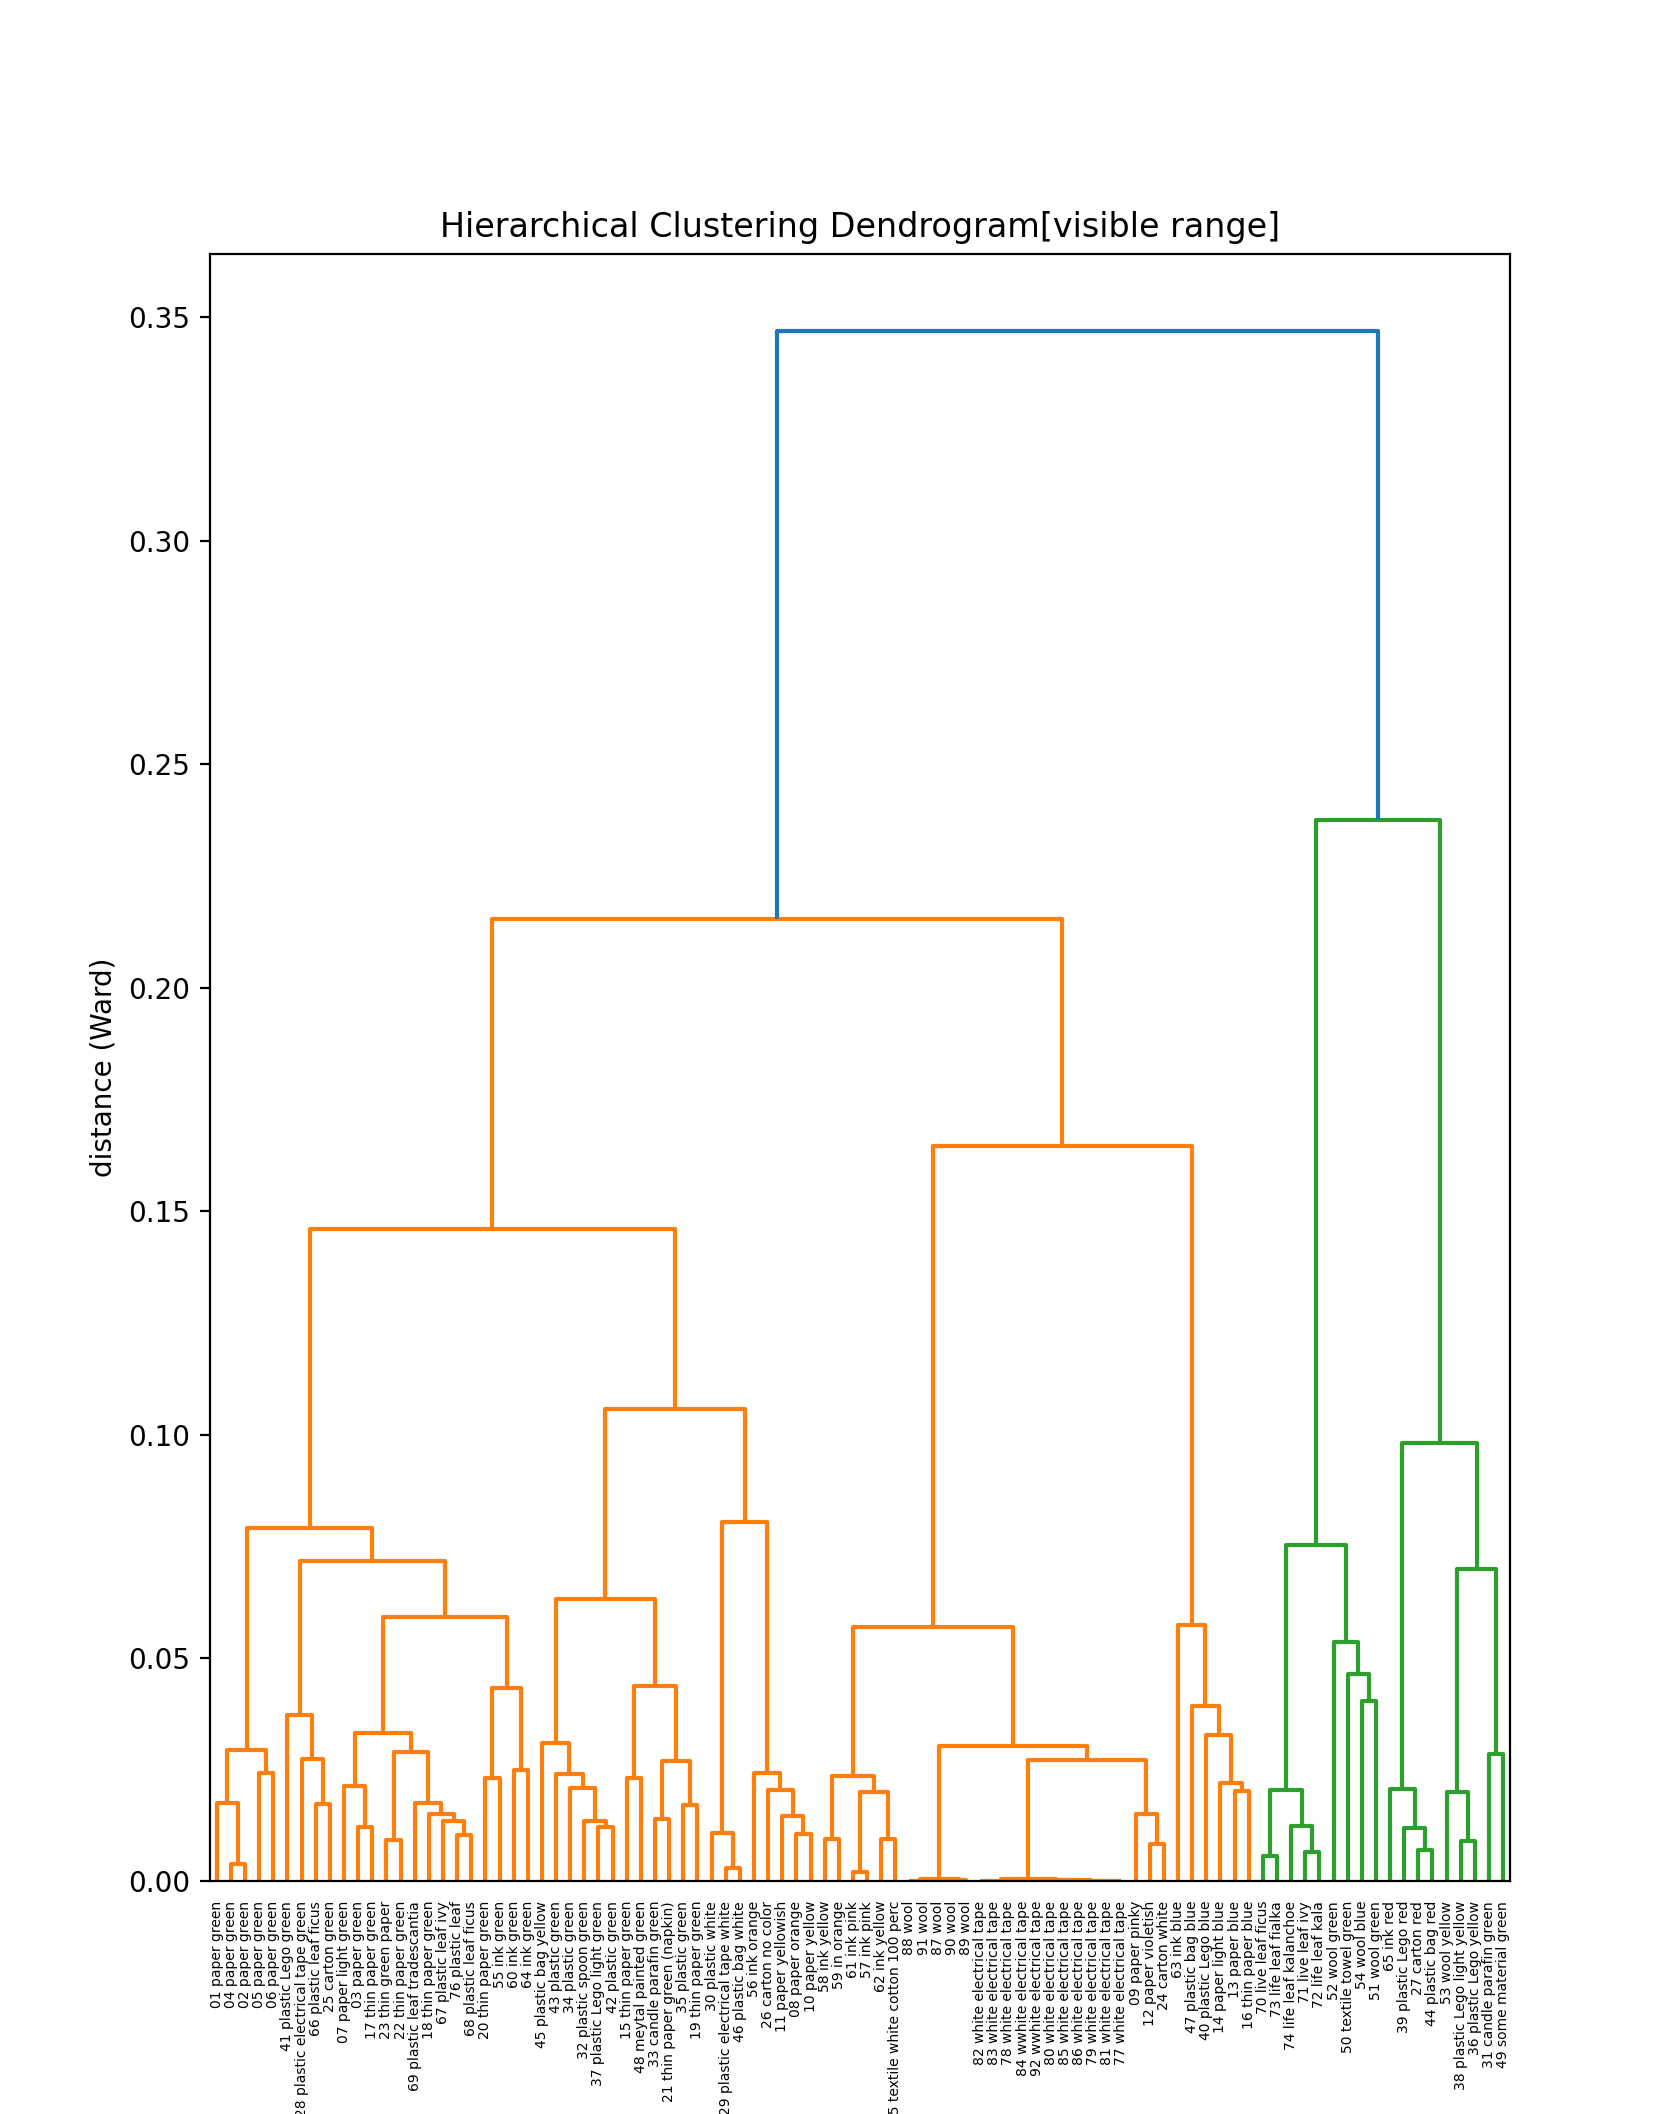
\includegraphics[width=0.65\textwidth]{figs-task2/cluster-visible.png}
  }
  \caption[]{Clustering of all materials in visible and infrared
  wavelength range}
  \label{fig:clustering}
\end{figure}

\subsection{Codes for task2}

\begin{lstlisting}[language=python, caption=Code for compare two materials, label={code:compare-materials}]
from pathlib import Path
from random import shuffle

import matplotlib.pyplot as plt
import pandas as pd

csv_root = path_config.lectures / "LectureExercise #1, CSV/csv files"

def filter_path(names: list[str]):
    path_list = list(csv_root.glob("*.csv"))
    path_list = [path.stem.replace(".", " ") for path in csv_root.glob("*.csv")]

    for _name in names:
        name = " " + _name + " "
        path_list = list(filter(lambda x: name in x, path_list))
    path_list = [name.replace(" ", "*") + ".csv" for name in path_list]
    found = []
    for pathname in path_list:
        found.extend(list(csv_root.glob(pathname)))
    return found

def plot_2materials(path1: Path, path2: Path):
    _fig, ax = plt.subplots()

    name1 = path1.stem.split(".")[0]
    df1 = pd.read_csv(path1)
    x = df1["nm"]
    y = df1[" %R"]
    ax.plot(x, y, label=name1)

    name2 = path2.stem.split(".")[0]
    df2 = pd.read_csv(path2)
    x = df2["nm"]
    y = df2[" %R"]
    ax.plot(x, y, label=name2)

    ax.set_title(f"{name1} vs {name2}")
    ax.set_xlabel("Wavelength [nm]")
    ax.set_ylabel("Refrectance [0-100]%")
    ax.set_ylim(0, 100)
    ax.legend()

def plot_2materials_subtract(path1: Path, path2: Path):
    _fig, ax = plt.subplots()

    df1 = pd.read_csv(path1)
    x = df1["nm"]
    y1 = df1[" %R"]

    df2 = pd.read_csv(path2)
    y2 = df2[" %R"]

    ax.plot(x, y1 - y2)
    name1 = path1.stem.split(".")[0]
    name2 = path2.stem.split(".")[0]
    ax.set_title(f"{name1} - {name2}")
    ax.set_xlabel("Wavelength [nm]")
    ax.set_ylabel("Refrectance [0-100]%")

# compare two materials
paths1 = filter_path(["green", "paper"])
shuffle(paths1)
paths2 = filter_path(["yellow", "paper"])
shuffle(paths2)
plot_2materials(paths1[0], paths2[0])

# compare two materials
paths1 = filter_path(["thin green", "paper"])
shuffle(paths1)
paths2 = filter_path(["green", "paper"])
shuffle(paths2)
plot_2materials(paths1[0], paths2[0])

# plot subtraction of two materials

paths = filter_path(["plastic", "green"])
shuffle(paths)
path1 = paths[0]

paths = filter_path(["paper", "green"])
shuffle(paths)
path2 = paths[0]
plot_2materials_subtract(path1, path2)

\end{lstlisting}


\begin{lstlisting}[language=python, caption=Code for clustering all materials, label={code:cluster-materials}]
import matplotlib.pyplot as plt
import numpy as np
import pandas as pd
from scipy.cluster.hierarchy import dendrogram, linkage

from asi import path_config
from asi.utils import search_closest_index

csv_root = path_config.lectures / "LectureExercise #1, CSV/csv files"


labels = []
arrays = []
_df = pd.read_csv(next(csv_root.glob("*.csv")))
wavelengths = _df["nm"]
for path in list(csv_root.glob("*.csv")):
    label = path.stem.split(".")[0]
    labels.append(label)
    df = pd.read_csv(path)
    assert df["nm"].equals(wavelengths)
    arrays.append(df[" %R"].to_numpy())
all_spectra = np.array(arrays).T


visible_max = 760
wavelengths = _df["nm"].to_list()
visible_max_index = search_closest_index(wavelengths, visible_max)


# Cluster with visible wavelengths


visible_range = slice(visible_max_index, None)

visible_wl = wavelengths[visible_range]
visible_spectra = all_spectra[visible_range]

# normalize
visible_spectra = visible_spectra / visible_spectra.sum(axis=0)

fig, ax = plt.subplots()
ax.plot(visible_wl, visible_spectra)
ax.set_title("Normalized spectra of visible range")
ax.set_ylabel("Normalized reflectance")
ax.set_xlabel("Wavelength [nm]")
plt.show()


Z = linkage(visible_spectra.T, "ward")
fig, ax = plt.subplots()
ax.set_title("Hierarchical Clustering Dendrogram[visible range]")

# Plot axis labels
ax.set_xlabel("sample index")
ax.set_ylabel("distance (Ward)")

# Make the dendrogram
_ = dendrogram(Z, labels=labels, leaf_rotation=90, ax=ax)
plt.show()


# Cluster with IR wavelengths


ir_range = slice(0, visible_max)
ir_wl = wavelengths[ir_range]
ir_spectra = all_spectra[ir_range]
ir_spectrum = all_spectra[ir_range].sum(axis=0)

ir_range = slice(0, visible_max_index)

ir_wl = wavelengths[ir_range]
ir_spectra = all_spectra[ir_range]

# normalize
ir_spectra = ir_spectra / ir_spectra.sum(axis=0)

fig, ax = plt.subplots()
ax.plot(ir_wl, ir_spectra)
ax.set_title("Normalized spectra of IR range")
ax.set_ylabel("Normalized reflectance")
ax.set_xlabel("Wavelength [nm]")
plt.show()


Z = linkage(ir_spectra.T, "ward")
fig, ax = plt.subplots(tight_layout=True, figsize=(10, 8))
ax.set_title("Hierarchical Clustering Dendrogram [IR range]")

# Plot axis labels
ax.set_xlabel("sample index")
ax.set_ylabel("distance (Ward)")

# Make the dendrogram
_ = dendrogram(Z, labels=labels, leaf_rotation=90, ax=ax)
plt.show()
\end{lstlisting}

